

\tikzset{every picture/.style={line width=0.75pt}} %set default line width to 0.75pt        

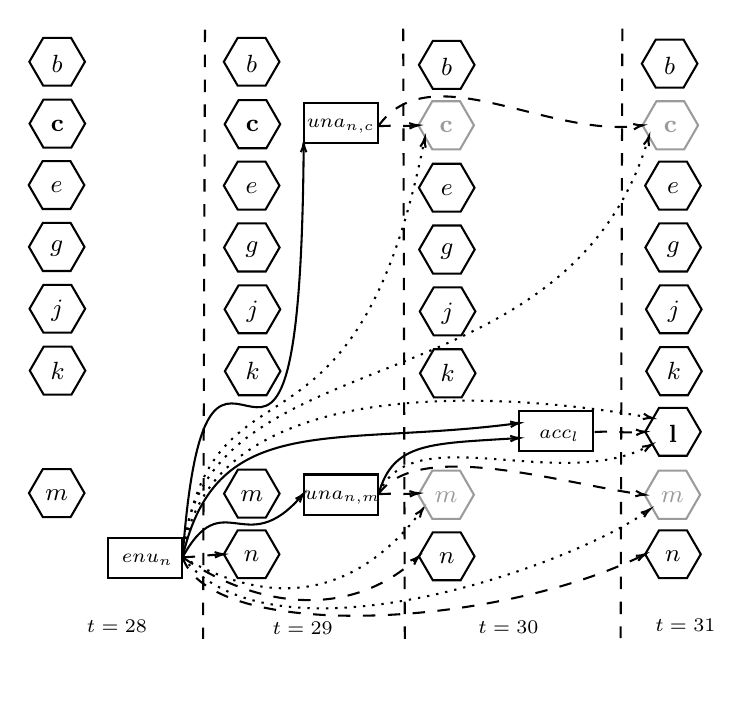
\begin{tikzpicture}[x=0.75pt,y=0.75pt,yscale=-1,xscale=1]
%uncomment if require: \path (0,300); %set diagram left start at 0, and has height of 300

%Shape: Rectangle [id:dp32394197299921523] 
\draw  [line width=0.75]  (38.8,251.2) -- (74.6,251.2) -- (74.6,270.54) -- (38.8,270.54) -- cycle ;
%Straight Lines [id:da5103454315814933] 
\draw  [dash pattern={on 4.5pt off 4.5pt}]  (85.53,6.3) -- (84.6,299.8) ;
%Straight Lines [id:da9625799604219181] 
\draw  [dash pattern={on 4.5pt off 4.5pt}]  (181.03,5.8) -- (181.8,299.8) ;
%Straight Lines [id:da937826652519754] 
\draw  [dash pattern={on 4.5pt off 4.5pt}]  (286.6,5.8) -- (285.8,299.4) ;
%Shape: Rectangle [id:dp39055029505322625] 
\draw  [line width=0.75]  (133.09,41.57) -- (168.89,41.57) -- (168.89,60.91) -- (133.09,60.91) -- cycle ;
%Shape: Polygon [id:dp25831662543105294] 
\draw   (27.7,21.73) -- (21,33.26) -- (7.6,33.26) -- (0.91,21.73) -- (7.6,10.19) -- (21,10.19) -- cycle ;
%Shape: Polygon [id:dp17264867524000027] 
\draw   (121.4,21.73) -- (114.7,33.26) -- (101.3,33.26) -- (94.6,21.73) -- (101.3,10.19) -- (114.7,10.19) -- cycle ;
%Shape: Polygon [id:dp9933858680624272] 
\draw   (215.4,23.23) -- (208.7,34.76) -- (195.3,34.76) -- (188.6,23.23) -- (195.3,11.69) -- (208.7,11.69) -- cycle ;
%Shape: Rectangle [id:dp8416513794122603] 
\draw  [line width=0.75]  (236.69,189.97) -- (272.49,189.97) -- (272.49,209.31) -- (236.69,209.31) -- cycle ;
%Curve Lines [id:da03689428077806867] 
\draw  [dash pattern={on 4.5pt off 4.5pt}]  (74.74,260.46) .. controls (110.24,284.75) and (154.9,290.88) .. (187.62,260.92) ;
\draw [shift={(188.6,260)}, rotate = 136.62] [color={rgb, 255:red, 0; green, 0; blue, 0 }  ][line width=0.75]    (4.37,-1.32) .. controls (2.78,-0.56) and (1.32,-0.12) .. (0,0) .. controls (1.32,0.12) and (2.78,0.56) .. (4.37,1.32)   ;
%Curve Lines [id:da9511759619364188] 
\draw    (74.74,260.46) .. controls (94.3,224.74) and (104.69,262.24) .. (131.75,231.26) ;
\draw [shift={(133,229.8)}, rotate = 129.81] [color={rgb, 255:red, 0; green, 0; blue, 0 }  ][line width=0.75]    (4.37,-1.32) .. controls (2.78,-0.56) and (1.32,-0.12) .. (0,0) .. controls (1.32,0.12) and (2.78,0.56) .. (4.37,1.32)   ;
%Shape: Regular Polygon [id:dp0962459706720944] 
\draw  [color={rgb, 255:red, 155; green, 155; blue, 155 }  ,draw opacity=1 ] (215.1,52.33) -- (208.41,63.92) -- (195.03,63.92) -- (188.34,52.33) -- (195.03,40.75) -- (208.41,40.75) -- cycle ;
%Curve Lines [id:da23781812589748064] 
\draw  [dash pattern={on 0.84pt off 2.51pt}]  (74.74,260.46) .. controls (136.15,295.88) and (173.1,260.09) .. (189.61,238.31) ;
\draw [shift={(190.6,237)}, rotate = 126.53] [color={rgb, 255:red, 0; green, 0; blue, 0 }  ][line width=0.75]    (4.37,-1.32) .. controls (2.78,-0.56) and (1.32,-0.12) .. (0,0) .. controls (1.32,0.12) and (2.78,0.56) .. (4.37,1.32)   ;
%Shape: Regular Polygon [id:dp5863365292722718] 
\draw   (27.78,51.53) -- (21.09,63.12) -- (7.71,63.12) -- (1.02,51.53) -- (7.71,39.95) -- (21.09,39.95) -- cycle ;
%Shape: Polygon [id:dp668166576601705] 
\draw   (27.4,81.13) -- (20.7,92.66) -- (7.3,92.66) -- (0.6,81.13) -- (7.3,69.59) -- (20.7,69.59) -- cycle ;
%Shape: Regular Polygon [id:dp1615790376024172] 
\draw   (27.48,110.93) -- (20.79,122.52) -- (7.41,122.52) -- (0.72,110.93) -- (7.41,99.35) -- (20.79,99.35) -- cycle ;
%Shape: Polygon [id:dp5652109778432169] 
\draw   (27.8,140.73) -- (21.1,152.26) -- (7.7,152.26) -- (1,140.73) -- (7.7,129.19) -- (21.1,129.19) -- cycle ;
%Shape: Regular Polygon [id:dp5554624960747061] 
\draw   (27.88,170.53) -- (21.19,182.12) -- (7.81,182.12) -- (1.12,170.53) -- (7.81,158.95) -- (21.19,158.95) -- cycle ;
%Shape: Regular Polygon [id:dp13320010668351145] 
\draw   (27.48,229.53) -- (20.79,241.12) -- (7.41,241.12) -- (0.72,229.53) -- (7.41,217.95) -- (20.79,217.95) -- cycle ;
%Shape: Regular Polygon [id:dp33133807114366276] 
\draw   (121.78,51.8) -- (115.09,63.39) -- (101.71,63.39) -- (95.02,51.8) -- (101.71,40.22) -- (115.09,40.22) -- cycle ;
%Shape: Polygon [id:dp7206917082119544] 
\draw   (121.4,81.4) -- (114.7,92.94) -- (101.3,92.94) -- (94.6,81.4) -- (101.3,69.86) -- (114.7,69.86) -- cycle ;
%Shape: Regular Polygon [id:dp689513993897114] 
\draw   (121.48,111.2) -- (114.79,122.79) -- (101.41,122.79) -- (94.72,111.2) -- (101.41,99.62) -- (114.79,99.62) -- cycle ;
%Shape: Polygon [id:dp3553082836345921] 
\draw   (121.8,141) -- (115.1,152.54) -- (101.7,152.54) -- (95,141) -- (101.7,129.46) -- (115.1,129.46) -- cycle ;
%Shape: Regular Polygon [id:dp08808706934177946] 
\draw   (121.88,170.8) -- (115.19,182.39) -- (101.81,182.39) -- (95.12,170.8) -- (101.81,159.22) -- (115.19,159.22) -- cycle ;
%Shape: Regular Polygon [id:dp3825724531298007] 
\draw   (121.48,229.8) -- (114.79,241.39) -- (101.41,241.39) -- (94.72,229.8) -- (101.41,218.22) -- (114.79,218.22) -- cycle ;
%Shape: Polygon [id:dp6015095613297166] 
\draw   (121.4,259) -- (114.7,270.54) -- (101.3,270.54) -- (94.6,259) -- (101.3,247.46) -- (114.7,247.46) -- cycle ;
%Shape: Polygon [id:dp9730868685192309] 
\draw   (215.4,82.4) -- (208.7,93.94) -- (195.3,93.94) -- (188.6,82.4) -- (195.3,70.86) -- (208.7,70.86) -- cycle ;
%Shape: Regular Polygon [id:dp04394747212171679] 
\draw   (215.48,112.2) -- (208.79,123.79) -- (195.41,123.79) -- (188.72,112.2) -- (195.41,100.62) -- (208.79,100.62) -- cycle ;
%Shape: Polygon [id:dp625486130912703] 
\draw   (215.8,142) -- (209.1,153.54) -- (195.7,153.54) -- (189,142) -- (195.7,130.46) -- (209.1,130.46) -- cycle ;
%Shape: Regular Polygon [id:dp6973070301209515] 
\draw   (215.88,171.8) -- (209.19,183.39) -- (195.81,183.39) -- (189.12,171.8) -- (195.81,160.22) -- (209.19,160.22) -- cycle ;
%Shape: Polygon [id:dp15730100429007365] 
\draw   (215.4,260) -- (208.7,271.54) -- (195.3,271.54) -- (188.6,260) -- (195.3,248.46) -- (208.7,248.46) -- cycle ;
%Shape: Polygon [id:dp7669928381847199] 
\draw   (324.4,81.4) -- (317.7,92.94) -- (304.3,92.94) -- (297.6,81.4) -- (304.3,69.86) -- (317.7,69.86) -- cycle ;
%Shape: Regular Polygon [id:dp8720689089102229] 
\draw   (324.48,111.2) -- (317.79,122.79) -- (304.41,122.79) -- (297.72,111.2) -- (304.41,99.62) -- (317.79,99.62) -- cycle ;
%Shape: Polygon [id:dp8686588781646976] 
\draw   (324.8,141) -- (318.1,152.54) -- (304.7,152.54) -- (298,141) -- (304.7,129.46) -- (318.1,129.46) -- cycle ;
%Shape: Regular Polygon [id:dp58257999600958] 
\draw   (324.88,170.8) -- (318.19,182.39) -- (304.81,182.39) -- (298.12,170.8) -- (304.81,159.22) -- (318.19,159.22) -- cycle ;
%Shape: Polygon [id:dp5246042913035425] 
\draw   (324.4,200) -- (317.7,211.54) -- (304.3,211.54) -- (297.6,200) -- (304.3,188.46) -- (317.7,188.46) -- cycle ;
%Shape: Polygon [id:dp40275693353577746] 
\draw   (324.4,259) -- (317.7,270.54) -- (304.3,270.54) -- (297.6,259) -- (304.3,247.46) -- (317.7,247.46) -- cycle ;
%Shape: Rectangle [id:dp294546304037402] 
\draw  [line width=0.75]  (133.09,220.57) -- (168.89,220.57) -- (168.89,239.91) -- (133.09,239.91) -- cycle ;
%Shape: Regular Polygon [id:dp13124017670187849] 
\draw  [color={rgb, 255:red, 155; green, 155; blue, 155 }  ,draw opacity=1 ] (323.1,52.33) -- (316.41,63.92) -- (303.03,63.92) -- (296.34,52.33) -- (303.03,40.75) -- (316.41,40.75) -- cycle ;
%Shape: Regular Polygon [id:dp6955758409780655] 
\draw  [color={rgb, 255:red, 155; green, 155; blue, 155 }  ,draw opacity=1 ] (215.1,230.33) -- (208.41,241.92) -- (195.03,241.92) -- (188.34,230.33) -- (195.03,218.75) -- (208.41,218.75) -- cycle ;
%Shape: Regular Polygon [id:dp41515587858602165] 
\draw  [color={rgb, 255:red, 155; green, 155; blue, 155 }  ,draw opacity=1 ] (324.1,230.33) -- (317.41,241.92) -- (304.03,241.92) -- (297.34,230.33) -- (304.03,218.75) -- (317.41,218.75) -- cycle ;
%Curve Lines [id:da9290568647401355] 
\draw    (74.74,260.46) .. controls (87.4,89) and (131.4,305) .. (133.09,60.91) ;
\draw [shift={(133.09,60.91)}, rotate = 90.4] [color={rgb, 255:red, 0; green, 0; blue, 0 }  ][line width=0.75]    (4.37,-1.32) .. controls (2.78,-0.56) and (1.32,-0.12) .. (0,0) .. controls (1.32,0.12) and (2.78,0.56) .. (4.37,1.32)   ;
%Curve Lines [id:da0024038948177537156] 
\draw    (74.74,260.46) .. controls (90.92,188.96) and (147.23,207.61) .. (235.66,195.98) ;
\draw [shift={(237,195.8)}, rotate = 172.34] [color={rgb, 255:red, 0; green, 0; blue, 0 }  ][line width=0.75]    (4.37,-1.32) .. controls (2.78,-0.56) and (1.32,-0.12) .. (0,0) .. controls (1.32,0.12) and (2.78,0.56) .. (4.37,1.32)   ;
%Curve Lines [id:da9423544130706317] 
\draw    (169.14,230.06) .. controls (176.09,204.98) and (193.66,205.77) .. (235.09,203.12) ;
\draw [shift={(237,203)}, rotate = 176.26] [color={rgb, 255:red, 0; green, 0; blue, 0 }  ][line width=0.75]    (4.37,-1.32) .. controls (2.78,-0.56) and (1.32,-0.12) .. (0,0) .. controls (1.32,0.12) and (2.78,0.56) .. (4.37,1.32)   ;
%Curve Lines [id:da07687685155568191] 
\draw  [dash pattern={on 4.5pt off 4.5pt}]  (74.74,260.46) .. controls (88.13,300.8) and (222.84,295.45) .. (296.5,259.54) ;
\draw [shift={(297.6,259)}, rotate = 153.62] [color={rgb, 255:red, 0; green, 0; blue, 0 }  ][line width=0.75]    (4.37,-1.32) .. controls (2.78,-0.56) and (1.32,-0.12) .. (0,0) .. controls (1.32,0.12) and (2.78,0.56) .. (4.37,1.32)   ;
%Curve Lines [id:da17080960388415456] 
\draw  [dash pattern={on 4.5pt off 4.5pt}]  (74.74,260.46) .. controls (88.36,259.78) and (80.46,259.9) .. (92.73,259.12) ;
\draw [shift={(94.6,259)}, rotate = 176.49] [color={rgb, 255:red, 0; green, 0; blue, 0 }  ][line width=0.75]    (4.37,-1.32) .. controls (2.78,-0.56) and (1.32,-0.12) .. (0,0) .. controls (1.32,0.12) and (2.78,0.56) .. (4.37,1.32)   ;
%Curve Lines [id:da6369256315030506] 
\draw  [dash pattern={on 4.5pt off 4.5pt}]  (169,52.78) .. controls (182.62,52.1) and (174.24,53.15) .. (186.47,52.44) ;
\draw [shift={(188.34,52.33)}, rotate = 176.49] [color={rgb, 255:red, 0; green, 0; blue, 0 }  ][line width=0.75]    (4.37,-1.32) .. controls (2.78,-0.56) and (1.32,-0.12) .. (0,0) .. controls (1.32,0.12) and (2.78,0.56) .. (4.37,1.32)   ;
%Curve Lines [id:da5460890529535121] 
\draw  [dash pattern={on 4.5pt off 4.5pt}]  (169.14,230.06) .. controls (182.76,229.38) and (174.38,230.43) .. (186.61,229.73) ;
\draw [shift={(188.48,229.62)}, rotate = 176.49] [color={rgb, 255:red, 0; green, 0; blue, 0 }  ][line width=0.75]    (4.37,-1.32) .. controls (2.78,-0.56) and (1.32,-0.12) .. (0,0) .. controls (1.32,0.12) and (2.78,0.56) .. (4.37,1.32)   ;
%Curve Lines [id:da9866128326016497] 
\draw  [dash pattern={on 4.5pt off 4.5pt}]  (169.14,230.06) .. controls (187.91,203.01) and (256.5,224.73) .. (295.58,230.1) ;
\draw [shift={(297.34,230.33)}, rotate = 187.26] [color={rgb, 255:red, 0; green, 0; blue, 0 }  ][line width=0.75]    (4.37,-1.32) .. controls (2.78,-0.56) and (1.32,-0.12) .. (0,0) .. controls (1.32,0.12) and (2.78,0.56) .. (4.37,1.32)   ;
%Curve Lines [id:da3372282256776671] 
\draw  [dash pattern={on 4.5pt off 4.5pt}]  (169,52.78) .. controls (193.95,17.75) and (250.26,58.57) .. (294.99,52.53) ;
\draw [shift={(296.34,52.33)}, rotate = 171.06] [color={rgb, 255:red, 0; green, 0; blue, 0 }  ][line width=0.75]    (4.37,-1.32) .. controls (2.78,-0.56) and (1.32,-0.12) .. (0,0) .. controls (1.32,0.12) and (2.78,0.56) .. (4.37,1.32)   ;
%Curve Lines [id:da7931620072938754] 
\draw  [dash pattern={on 4.5pt off 4.5pt}]  (273.22,200.11) .. controls (286.84,199.43) and (283.06,200.78) .. (295.7,200.11) ;
\draw [shift={(297.6,200)}, rotate = 176.49] [color={rgb, 255:red, 0; green, 0; blue, 0 }  ][line width=0.75]    (4.37,-1.32) .. controls (2.78,-0.56) and (1.32,-0.12) .. (0,0) .. controls (1.32,0.12) and (2.78,0.56) .. (4.37,1.32)   ;
%Curve Lines [id:da3170103066051301] 
\draw  [dash pattern={on 0.84pt off 2.51pt}]  (74.74,260.46) .. controls (118.16,315.64) and (262.47,264.45) .. (298.73,238.19) ;
\draw [shift={(299.8,237.4)}, rotate = 142.92] [color={rgb, 255:red, 0; green, 0; blue, 0 }  ][line width=0.75]    (4.37,-1.32) .. controls (2.78,-0.56) and (1.32,-0.12) .. (0,0) .. controls (1.32,0.12) and (2.78,0.56) .. (4.37,1.32)   ;
%Curve Lines [id:da2974445519606693] 
\draw  [dash pattern={on 0.84pt off 2.51pt}]  (74.74,260.46) .. controls (87.54,158.68) and (268.35,187.37) .. (299.3,193.08) ;
\draw [shift={(301,193.4)}, rotate = 190.78] [color={rgb, 255:red, 0; green, 0; blue, 0 }  ][line width=0.75]    (4.37,-1.32) .. controls (2.78,-0.56) and (1.32,-0.12) .. (0,0) .. controls (1.32,0.12) and (2.78,0.56) .. (4.37,1.32)   ;
%Curve Lines [id:da007173676928789563] 
\draw  [dash pattern={on 0.84pt off 2.51pt}]  (74.74,260.46) .. controls (87.8,155) and (157.8,229.8) .. (191.4,58.6) ;
\draw [shift={(191.4,58.6)}, rotate = 101.1] [color={rgb, 255:red, 0; green, 0; blue, 0 }  ][line width=0.75]    (4.37,-1.32) .. controls (2.78,-0.56) and (1.32,-0.12) .. (0,0) .. controls (1.32,0.12) and (2.78,0.56) .. (4.37,1.32)   ;
%Curve Lines [id:da8424571147503932] 
\draw  [dash pattern={on 0.84pt off 2.51pt}]  (74.74,260.46) .. controls (81.4,151.4) and (260.2,192.6) .. (299.4,57.8) ;
\draw [shift={(299.4,57.8)}, rotate = 106.21] [color={rgb, 255:red, 0; green, 0; blue, 0 }  ][line width=0.75]    (4.37,-1.32) .. controls (2.78,-0.56) and (1.32,-0.12) .. (0,0) .. controls (1.32,0.12) and (2.78,0.56) .. (4.37,1.32)   ;
%Curve Lines [id:da832051990599513] 
\draw  [dash pattern={on 0.84pt off 2.51pt}]  (169.14,230.06) .. controls (184.45,192.58) and (255.95,229.84) .. (299.3,206.91) ;
\draw [shift={(300.6,206.2)}, rotate = 150.54] [color={rgb, 255:red, 0; green, 0; blue, 0 }  ][line width=0.75]    (4.37,-1.32) .. controls (2.78,-0.56) and (1.32,-0.12) .. (0,0) .. controls (1.32,0.12) and (2.78,0.56) .. (4.37,1.32)   ;
%Shape: Polygon [id:dp822443066516893] 
\draw   (322.8,22.63) -- (316.1,34.16) -- (302.7,34.16) -- (296,22.63) -- (302.7,11.09) -- (316.1,11.09) -- cycle ;

% Text Node
\draw (27.13,289.4) node [anchor=north west][inner sep=0.75pt]  [font=\scriptsize]  {$t=28$};
% Text Node
\draw (44,257.6) node [anchor=north west][inner sep=0.75pt]  [font=\scriptsize]  {$enu_{n}$};
% Text Node
\draw (133.09,47.97) node [anchor=north west][inner sep=0.75pt]  [font=\scriptsize]  {$una_{n,c}$};
% Text Node
\draw (116.67,290.33) node [anchor=north west][inner sep=0.75pt]  [font=\scriptsize]  {$t=29$};
% Text Node
\draw (215.8,289.9) node [anchor=north west][inner sep=0.75pt]  [font=\scriptsize]  {$t=30$};
% Text Node
\draw (301,288.9) node [anchor=north west][inner sep=0.75pt]  [font=\scriptsize]  {$t=31$};
% Text Node
\draw (14.3,22.73) node  [font=\small]  {$b$};
% Text Node
\draw (108,22.73) node  [font=\small]  {$b$};
% Text Node
\draw (202,24.23) node  [font=\small]  {$b$};
% Text Node
\draw (245.19,197.57) node [anchor=north west][inner sep=0.75pt]  [font=\scriptsize]  {$acc_{l}$};
% Text Node
\draw (201.72,53.33) node  [font=\small,color={rgb, 255:red, 155; green, 155; blue, 155 }  ,opacity=1 ]  {$\mathbf{c}$};
% Text Node
\draw (14.4,52.53) node  [font=\small]  {$\mathbf{c}$};
% Text Node
\draw (14,82.13) node  [font=\small]  {$e$};
% Text Node
\draw (14.1,111.93) node  [font=\small]  {$g$};
% Text Node
\draw (14.4,141.73) node  [font=\small]  {$j$};
% Text Node
\draw (14.5,170.53) node  [font=\small]  {$k$};
% Text Node
\draw (14.1,230.53) node  [font=\small]  {$m$};
% Text Node
\draw (108.4,52.8) node  [font=\small]  {$\mathbf{c}$};
% Text Node
\draw (108,82.4) node  [font=\small]  {$e$};
% Text Node
\draw (108.1,112.2) node  [font=\small]  {$g$};
% Text Node
\draw (108.4,142) node  [font=\small]  {$j$};
% Text Node
\draw (108.5,170.8) node  [font=\small]  {$k$};
% Text Node
\draw (108.1,230.8) node  [font=\small]  {$m$};
% Text Node
\draw (108,260) node  [font=\small]  {$n$};
% Text Node
\draw (202,83.4) node  [font=\small]  {$e$};
% Text Node
\draw (202.1,113.2) node  [font=\small]  {$g$};
% Text Node
\draw (202.4,143) node  [font=\small]  {$j$};
% Text Node
\draw (202.5,171.8) node  [font=\small]  {$k$};
% Text Node
\draw (202,261) node  [font=\small]  {$n$};
% Text Node
\draw (311,82.4) node  [font=\small]  {$e$};
% Text Node
\draw (311.1,112.2) node  [font=\small]  {$g$};
% Text Node
\draw (311.4,142) node  [font=\small]  {$j$};
% Text Node
\draw (311.5,170.8) node  [font=\small]  {$k$};
% Text Node
\draw (311,201) node  [font=\small]  {$\mathbf{l}$};
% Text Node
\draw (311,260) node  [font=\small]  {$n$};
% Text Node
\draw (132.09,226.97) node [anchor=north west][inner sep=0.75pt]  [font=\scriptsize]  {$una_{n,m}$};
% Text Node
\draw (309.72,53.33) node  [font=\small,color={rgb, 255:red, 155; green, 155; blue, 155 }  ,opacity=1 ]  {$\mathbf{c}$};
% Text Node
\draw (201.72,231.33) node  [font=\small,color={rgb, 255:red, 155; green, 155; blue, 155 }  ,opacity=1 ]  {$m$};
% Text Node
\draw (310.72,231.33) node  [font=\small,color={rgb, 255:red, 155; green, 155; blue, 155 }  ,opacity=1 ]  {$m$};
% Text Node
\draw (309.4,23.63) node  [font=\small]  {$b$};


\end{tikzpicture}
